\documentclass{article}

\usepackage{arxiv}

\usepackage[utf8]{inputenc} % allow utf-8 input
\usepackage[T1]{fontenc}    % use 8-bit T1 fonts
\usepackage{lmodern}        % https://github.com/rstudio/rticles/issues/343
\usepackage{hyperref}       % hyperlinks
\usepackage{url}            % simple URL typesetting
\usepackage{booktabs}       % professional-quality tables
\usepackage{amsfonts}       % blackboard math symbols
\usepackage{nicefrac}       % compact symbols for 1/2, etc.
\usepackage{microtype}      % microtypography
\usepackage{lipsum}
\usepackage{graphicx}

\title{Vaccinating Australia: How long will it take?}

\author{
    Mark Hanly
   \\
    Centre for Big Data Research in Health \\
    UNSW Sydney \\
   \\
  \texttt{\href{mailto:m.hanly@unsw.edu.au}{\nolinkurl{m.hanly@unsw.edu.au}}} \\
   \And
    Tim Churches
   \\
    South Western Sydney Clinical School, Faculty of Medicine \& Health,
UNSW Sydney \& \\
    Ingham Institute for Applied Medical Research \\
   \\
  \texttt{\href{mailto:timothy.churches@unsw.edu.au}{\nolinkurl{timothy.churches@unsw.edu.au}}} \\
   \And
    Oisín Fitzgerald
   \\
    Centre for Big Data Research in Health \\
    UNSW Sydney \\
   \\
  \texttt{\href{mailto:o.fitzgerald@unsw.edu.au}{\nolinkurl{o.fitzgerald@unsw.edu.au}}} \\
   \And
    C Raina McIntyre
   \\
    Biosecurity Research Program, The Kirby Institute \\
    UNSW Sydney \\
   \\
  \texttt{\href{mailto:rainam@protonmail.com}{\nolinkurl{rainam@protonmail.com}}} \\
   \And
    Louisa Jorm
   \\
    Centre for Big Data Research in Health \\
    UNSW Sydney \\
   \\
  \texttt{\href{mailto:l.jorm@unsw.edu.au}{\nolinkurl{l.jorm@unsw.edu.au}}} \\
  }


% Pandoc citation processing
\newlength{\csllabelwidth}
\setlength{\csllabelwidth}{3em}
\newlength{\cslhangindent}
\setlength{\cslhangindent}{1.5em}
% for Pandoc 2.8 to 2.10.1
\newenvironment{cslreferences}%
  {}%
  {\par}
% For Pandoc 2.11+
\newenvironment{CSLReferences}[3] % #1 hanging-ident, #2 entry spacing
 {% don't indent paragraphs
  \setlength{\parindent}{0pt}
  % turn on hanging indent if param 1 is 1
  \ifodd #1 \everypar{\setlength{\hangindent}{\cslhangindent}}\ignorespaces\fi
  % set entry spacing
  \ifnum #2 > 0
  \setlength{\parskip}{#2\baselineskip}
  \fi
 }%
 {}
\usepackage{calc} % for calculating minipage widths
\newcommand{\CSLBlock}[1]{#1\hfill\break}
\newcommand{\CSLLeftMargin}[1]{\parbox[t]{\csllabelwidth}{#1}}
\newcommand{\CSLRightInline}[1]{\parbox[t]{\linewidth - \csllabelwidth}{#1}}
\newcommand{\CSLIndent}[1]{\hspace{\cslhangindent}#1}

\usepackage[british]{babel}
\usepackage{gensymb}
\usepackage{booktabs}
\usepackage{longtable}
\usepackage{array}
\usepackage{multirow}
\usepackage{wrapfig}
\usepackage{float}
\usepackage{colortbl}
\usepackage{pdflscape}
\usepackage{tabu}
\usepackage{threeparttable}
\usepackage{threeparttablex}
\usepackage[normalem]{ulem}
\usepackage{makecell}
\usepackage{xcolor}


\begin{document}
\maketitle

\def\tightlist{}


\begin{abstract}
The Australian Government's COVID-19 vaccine rollout strategy is
scheduled to commence in late February 2021 and aims to vaccinate the
Australian adult population by the end of October 2021. The task of
vaccinating some 20 million people within this timeframe presents
considerable logistical challenges. Key to meeting this target is the
rate of vaccine delivery: the number of vaccine doses that can be
administered per day. In the opening phase, high priority groups will
receive the Pfizer/BioNTech vaccine through hospital hubs at an initial
rate of 80,000 doses per week. However, pending regulatory approval, the
currently announced plan appears to be to distribute the AstraZeneca
vaccine to the bulk of the popluation through a combination of general
practices and community pharmacies. Here, we run a series of projections
to estimate how long it will take to vaccinate the Australian population
under different assumptions about the rate of vaccine administration as
well as the schedule for second doses and prevalence of vaccine
hesitancy. Our analysis highlights the ambitious rate of vaccine
administration that will be neccessary to meet the Australian Government
completion target of October 2021. A rate of 200,000 doses per day would
comfortably meet that target; 80,000 doses a day would see roll-out
extended until mid-2022. Speed is of the essence when it comes to
vaccine rollout: protecting the population quickly will minimise the
risk of sporadic and costly lockdowns lockdowns and the potential for
small, local clusters getting out of control and sparking new epidemic
waves. The government should gather all its resources to maximise the
daily vaccination rate, ideally aiming to ramp up administration to at
least 200,000 doses per day as quickly as possible. Quickly achieving
and maintaining this pace will likely require dedicated large-scale
vaccination sites that are capable of delivering thousands of doses a
week in addition to the enthusiastic participation of GP practices and
community pharmacies around the country. Lessons on the neccessary
logistical planning, including coordination of delivery,
ultra-cold-chain storage and staffing, can potentially be learned from
Israel, where between 7,000 and 20,000 vaccinations per million
population have been delivered daily throughout January.
\end{abstract}

\keywords{
    COVID19
   \and
    vaccination
  }

\newpage

\hypertarget{introduction}{%
\section{Introduction}\label{introduction}}

The development and regulatory approval of multiple safe and efficacious
COVID-19 vaccines in less than a year is a truly remarkable achievement.
The logistical task of administering the vaccine rapidly and fairly to
billions of people around the world will be no less of a challenge.
National vaccination programs have commenced in many countries including
Israel, the United States and the United Kingdom. In Australia, the
federal government has entered into four agreements for the supply of
COVID-19 vaccines (Table \ref{tab:agreements}), with a view to starting
distribution in late February 2021, and setting an ambitious target of
completion of vaccination of the adult population in October
2021.\textsuperscript{1} This target allows just 35 weeks to administer
two doses each to some 20 million adult Australians.

\begin{table}[H]

\begin{threeparttable}
\caption{\label{tab:agreements}Vaccine supply agreements entered into by the Australian government}
\centering
\begin{tabular}[t]{>{\raggedright\arraybackslash}p{3cm}>{\raggedright\arraybackslash}p{3cm}>{\centering\arraybackslash}p{2cm}>{\raggedright\arraybackslash}p{2cm}>{\raggedright\arraybackslash}p{4cm}}
\toprule
Name & Type & Doses (millions) & Schedule & Status as at 1st February, 2021\\
\midrule
\cellcolor{gray!6}{Pfizer/BioNTech} & \cellcolor{gray!6}{mRNA vaccine} & \cellcolor{gray!6}{10} & \cellcolor{gray!6}{2 doses, 21 days apart} & \cellcolor{gray!6}{Provisionally approved by the TGA}\\
University of Oxford AstraZeneca & Viral vector vaccine & 54 & 2 doses, 28 days apart & Phase 3 clinical trials\\
\cellcolor{gray!6}{Novavax} & \cellcolor{gray!6}{Protein vaccine} & \cellcolor{gray!6}{51} & \cellcolor{gray!6}{2 doses, 21 days apart} & \cellcolor{gray!6}{Phase 3 clinical trials}\\
COVAX Facility & Assorted & 25 & Assorted & Nine candidate vaccines in various clinical trial stages\\
\bottomrule
\end{tabular}
\begin{tablenotes}
\small
\item [] Adapted from https://www.health.gov.au/initiatives-and-programs/covid-19-vaccines/about-covid-19-vaccines/australias-vaccine-agreements
\end{tablenotes}
\end{threeparttable}
\end{table}

The national roll-out strategy divides the population into 16 groups,
organised into five distinct phases (Table \ref{tab:phases}). Hospital
hubs with access to -70\degree C ultra-cold-chain storage facilities
will administer the Pfizer/BioNTech vaccine to the highest priority
groups scheduled in Phase 1a, which includes border workers, frontline
healthcare staff, and aged care staff and residents.\textsuperscript{2}
Pending approval, the AstraZeneca vaccine would be administered to the
bulk of the adult population through a network of general practitioners
(GPs) and community pharmacies.

The Pfizer/BioNTech and AstraZeneca vaccines both require two doses---a
primer and a booster---which need to be delivered within a specified
time frame after the initial shot. This complicates roll-out as the
resources of specialised vaccine administration facilities, and
nominated general practices and pharmacies must be divided between
unprotected individuals waiting for their first injection and those who
have already been afforded some protection and who are returning for
their booster administration. Furthermore, the duration of protection
afforded by these vaccines is not yet well characterised, and
re-vaccination of some or all of the population may be required. We have
not included re-vaccination into the any of the scenarios examined in
this paper, at this stage.

\begin{table}[H]

\begin{threeparttable}
\caption{\label{tab:phases}Australia’s COVID-19 vaccine national roll-out strategy}
\centering
\begin{tabular}[t]{>{\raggedright\arraybackslash}p{1cm}>{\raggedright\arraybackslash}p{11cm}>{\raggedleft\arraybackslash}p{2cm}}
\toprule
Phase & Description & Size\\
\midrule
\textbf{\cellcolor{gray!6}{1a}} & \cellcolor{gray!6}{Quarantine \& border workers} & \cellcolor{gray!6}{70,000}\\
\textbf{1a} & Frontline health care workers & 100,000\\
\textbf{\cellcolor{gray!6}{1a}} & \cellcolor{gray!6}{Aged care and disability care staff} & \cellcolor{gray!6}{318,000}\\
\textbf{1a} & Aged care and disability care residents & 190,000\\
\textbf{\cellcolor{gray!6}{1b}} & \cellcolor{gray!6}{Elderly adults aged 80 years and over} & \cellcolor{gray!6}{1,045,000}\\
\textbf{1b} & Elderly adults aged 70-79 years & 1,858,000\\
\textbf{\cellcolor{gray!6}{1b}} & \cellcolor{gray!6}{Other health care workers} & \cellcolor{gray!6}{953,000}\\
\textbf{1b} & Aboriginal and Torres Strait Islander people aged 55 years and over & 87,000\\
\textbf{\cellcolor{gray!6}{1b}} & \cellcolor{gray!6}{Younger adults with an underlying medical condition} & \cellcolor{gray!6}{2,000,000}\\
\textbf{1b} & Critical and high risk workers & 196,000\\
\textbf{\cellcolor{gray!6}{2a}} & \cellcolor{gray!6}{Adults aged 60-69} & \cellcolor{gray!6}{2,650,000}\\
\textbf{2a} & Adults aged 50-59 & 3,080,000\\
\textbf{\cellcolor{gray!6}{2a}} & \cellcolor{gray!6}{Aboriginal and Torres Strait Islander people aged 18-54} & \cellcolor{gray!6}{387,000}\\
\textbf{2a} & Other critical and high risk workers & 453,000\\
\textbf{\cellcolor{gray!6}{2b}} & \cellcolor{gray!6}{Balance of adult population} & \cellcolor{gray!6}{6,643,000}\\
\textbf{3} & <18 if recommended & 5,670,000\\
\bottomrule
\end{tabular}
\begin{tablenotes}
\small
\item [] Adapted from https://www.health.gov.au/sites/default/files/documents/2021/01/australia-s-covid-19-vaccine-national-roll-out-strategy.pdf
\end{tablenotes}
\end{threeparttable}
\end{table}

Another unknown is the question of vaccine hesitancy, which refers to
delay in acceptance or complete refusal of vaccination, despite a
suitable vaccine being available and accessible.\textsuperscript{3}
Clearly, high levels of vaccine hesitancy would have the potential to
undermine efforts to establish adequate protection of the whole
population through herd immunity. An online survey of over 3,000
Australian adults undertaken in August 2020 asked respondents if they
would agree to vaccination for COVID-19 if a safe and effective vaccine
were available. The population-weighted responses were 5.5\%
\emph{definitely not}, 7.2\% \emph{probably not}, 28.7\% \emph{probably
yes} and 58.5\% \emph{definitely yes}.\textsuperscript{4}

When it comes to vaccine roll-out, speed is of the essence. Statistical
modelling has illustrated that epidemic duration, cases and deaths are
minimised dramatically as the number of available daily vaccinations
increases. In one modelling scenario, for example, increasing the daily
capacity by 25\% from 75,000 to 100,000 resulted in a 60\% reduction in
total cases and deaths.\textsuperscript{5} The Australian Prime Minister
has cited a schedule starting at 80,000 vaccinations per week and
scaling up from there.\textsuperscript{6} It is unclear what the peak
daily vaccination target is, but a simple ``back of the envelope''
calculation suggests that in order to vaccinate some 20 million adult
Australians twice in the eight months from the start of March 2021 to
the end of October 2021 would take in the order of
\(\frac{20,000,000}{8 \times 30} \times 2 \approx 167,000\) doses per
day.

The aim of this analysis is to estimate how long it might take to
administer the announced two-dose COVID-19 vaccine schedule to the
Australian population. We consider a variety of scenarios based on the
daily vaccine administration capacities, the timeframe between the first
and second doses and the scale of vaccine hesitancy in the population.
We conclude by comparing daily vaccine administration rates from
countries where vaccination programs are already underway.

\hypertarget{methods}{%
\section{Methods}\label{methods}}

\hypertarget{population-and-priority-groups}{%
\subsection{Population and priority
groups}\label{population-and-priority-groups}}

Our analysis is based on the 16 priority groups and five phases proposed
by the Australian government (see Table \ref{tab:phases}). The assumed
population size is 25.7 million people, including 5.67 million children
and adolescents under the age of 18. We also assume that equal priority
will be given to all groups within the same phase.

\hypertarget{vaccine-roll-out-projections}{%
\subsection{Vaccine roll out
projections}\label{vaccine-roll-out-projections}}

Roll out projections are based on three parameters:

\begin{enumerate}
\def\labelenumi{\arabic{enumi}.}
\tightlist
\item
  The daily vaccination capacity.
\item
  The valid window (in days) to receive the second dose after the first
  has been administered.
\item
  Vaccine hesitancy.
\end{enumerate}

\hypertarget{projection-scenarios}{%
\subsection{Projection scenarios}\label{projection-scenarios}}

Projection scenarios are based on a \(2^k\) factorial design defined by
three factors with two levels each. The scenarios are summarised in
Table \ref{tab:scenarios} and the three factors and levels are detailed
below:

\begin{itemize}
\item
  Daily vaccination capacity (80,000 versus 200,000)
\item
  Timing between first and second dose (3-6 weeks versus 3-12 weeks)
\item
  Vaccine hesitancy (7\% versus 13\%).
\end{itemize}

\begin{table}[H]

\caption{\label{tab:scenarios}Projection scenarios}
\centering
\begin{tabu} to \linewidth {>{}l>{\raggedleft}X>{\raggedleft}X>{\raggedleft}X}
\toprule
Scenario & Capacity (doses per day) & Gap between doses & Hesitancy\\
\midrule
\textbf{\cellcolor{gray!6}{1}} & \cellcolor{gray!6}{80,000} & \cellcolor{gray!6}{3 to 6 weeks} & \cellcolor{gray!6}{7\%}\\
\textbf{2} & 80,000 & 3 to 6 weeks & 13\%\\
\textbf{\cellcolor{gray!6}{3}} & \cellcolor{gray!6}{80,000} & \cellcolor{gray!6}{3 to 12 weeks} & \cellcolor{gray!6}{7\%}\\
\textbf{4} & 80,000 & 3 to 12 weeks & 13\%\\
\textbf{\cellcolor{gray!6}{5}} & \cellcolor{gray!6}{200,000} & \cellcolor{gray!6}{3 to 6 weeks} & \cellcolor{gray!6}{7\%}\\
\textbf{6} & 200,000 & 3 to 6 weeks & 13\%\\
\textbf{\cellcolor{gray!6}{7}} & \cellcolor{gray!6}{200,000} & \cellcolor{gray!6}{3 to 12 weeks} & \cellcolor{gray!6}{7\%}\\
\textbf{8} & 200,000 & 3 to 12 weeks & 13\%\\
\bottomrule
\end{tabu}
\end{table}

The projections assume that those who are hesitant will never receive
the vaccine. The specified hesitancy rates are based on the survey data
reported by Edwards \emph{et al.},\textsuperscript{4} and are only
applied to general population groups. Border staff, healthcare and aged
care workers, aged care residents and adults with a medical condition
were assumed to have negligible vaccine hesitancy.

\hypertarget{vaccine-allocation}{%
\subsection{Vaccine allocation}\label{vaccine-allocation}}

We allocated the daily available vaccination doses according to the
following algorithm:

\begin{enumerate}
\def\labelenumi{\arabic{enumi}.}
\item
  Calculate the number of second doses due, based on the specified
  permissible range for the second dose. As an example, if the second
  dose is specified to be administered at between three and six weeks,
  then the booster doses for people vaccinated on day 1 would be evenly
  distributed across the three weeks between day 22 and day 42).
\item
  Assign the remaining doses from the daily limit to those awaiting
  their first dose.
\item
  Identify the highest priority phase that hasn't yet received all first
  doses.
\item
  Divide the available first doses between the subgroups in the highest
  priority phase, proportional to the number of unvaccinated individuals
  remaining in each subgroup.
\item
  Stop when all population members, minus those who are hesitant, have
  been vaccinated twice.
\end{enumerate}

\hypertarget{software-and-code}{%
\subsection{Software and code}\label{software-and-code}}

The analysis was performed using R version 4.0.3\textsuperscript{7} and
associated packages\textsuperscript{8}. The complete source code to
reproduce this analysis can be accessed at
\url{https://github.com/CBDRH/vaccinatingAustralia}.

\hypertarget{results}{%
\section{Results}\label{results}}

Results from the eight scenarios are presented in Table
\ref{tab:scenarios}. Scenarios that assumed a vaccine hesitancy of 7\%
among the general population resulted in 48.3 million vaccine doses
administered to 24.2 million people, corresponding to a population
coverage of 94.0\%. Scenarios that assumed the vaccine higher hesitancy
rate of 13\% resulted in 45.7 million vaccine doses administered to 22.9
million people for a coverage of 88.9\%.

Under an optimistic Scenario of 200,000 daily doses with the 7\%
hesitancy rate (Scenario 5), assuming a start date of 1 March 2021,
Phase 1a would be fully vaccinated (i.e.~primer and booster doses
administered) as early as 13 April 2021---in just six elapsed weeks. The
entire adult population would be fully vaccinated by about 25 October
2021---in line with government targets---and a further eight weeks would
see the entire population include those under 18 vaccinated. Under this
optimistic scenario, the vulnerable groups in Phase 1b, including adults
aged 70 and above and those with underlying medical conditions, would be
fully vaccinated before the onset of the Southern Hemisphere winter.
Under this scenario, we would reach 50\% population coverage in late
July 2021 and 75\% population around the start of October 2021 (Figure
\ref{fig:cumlResults}A).

\begin{table}[H]

\caption{\label{tab:projections}Summary of vaccine roll-out projections for different scenarios}
\centering
\begin{tabu} to \linewidth {>{}l>{\raggedleft}X>{\raggedleft}X>{\raggedleft}X>{\raggedright}X>{\raggedright}X>{\raggedright}X>{\raggedright}X>{\raggedright}X}
\toprule
Scenario & Number of vaccine doses (millions) & Individuals vaccinated (millions) & Population coverage (\%) & Phase 1a complete & Phase 1b complete & Phase 2a complete & Phase 2b complete & Phase 3 complete\\
\midrule
\textbf{\cellcolor{gray!6}{1}} & \cellcolor{gray!6}{48.3} & \cellcolor{gray!6}{24.2} & \cellcolor{gray!6}{94.0} & \cellcolor{gray!6}{Apr2021} & \cellcolor{gray!6}{Sep2021} & \cellcolor{gray!6}{Feb2022} & \cellcolor{gray!6}{Jul2022} & \cellcolor{gray!6}{Nov2022}\\
\textbf{2} & 45.7 & 22.9 & 88.9 & Apr2021 & Sep2021 & Jan2022 & Jun2022 & Oct2022\\
\textbf{\cellcolor{gray!6}{3}} & \cellcolor{gray!6}{48.3} & \cellcolor{gray!6}{24.2} & \cellcolor{gray!6}{94.0} & \cellcolor{gray!6}{May2021} & \cellcolor{gray!6}{Oct2021} & \cellcolor{gray!6}{Mar2022} & \cellcolor{gray!6}{Aug2022} & \cellcolor{gray!6}{Dec2022}\\
\textbf{4} & 45.7 & 22.9 & 88.9 & May2021 & Oct2021 & Feb2022 & Jul2022 & Nov2022\\
\textbf{\cellcolor{gray!6}{5}} & \cellcolor{gray!6}{48.3} & \cellcolor{gray!6}{24.2} & \cellcolor{gray!6}{94.0} & \cellcolor{gray!6}{Apr2021} & \cellcolor{gray!6}{Jun2021} & \cellcolor{gray!6}{Aug2021} & \cellcolor{gray!6}{Oct2021} & \cellcolor{gray!6}{Dec2021}\\
\textbf{6} & 45.7 & 22.9 & 88.9 & Apr2021 & Jun2021 & Jul2021 & Sep2021 & Nov2021\\
\textbf{\cellcolor{gray!6}{7}} & \cellcolor{gray!6}{48.3} & \cellcolor{gray!6}{24.2} & \cellcolor{gray!6}{94.0} & \cellcolor{gray!6}{May2021} & \cellcolor{gray!6}{Jun2021} & \cellcolor{gray!6}{Sep2021} & \cellcolor{gray!6}{Oct2021} & \cellcolor{gray!6}{Dec2021}\\
\textbf{8} & 45.7 & 22.9 & 88.9 & May2021 & Jun2021 & Sep2021 & Oct2021 & Dec2021\\
\bottomrule
\end{tabu}
\end{table}

Under the less optimistic scenarios of 80,000 doses administered daily,
it would take until some time between June and August 2022 to vaccinate
the adult population (Table \ref{tab:scenarios}). Under Scenario 1, we
would reach 50\% population coverage in January 2022 and 75\% population
coverage in July 2022 (Figure \ref{fig:cumlResults}B).

\begin{figure}

{\centering 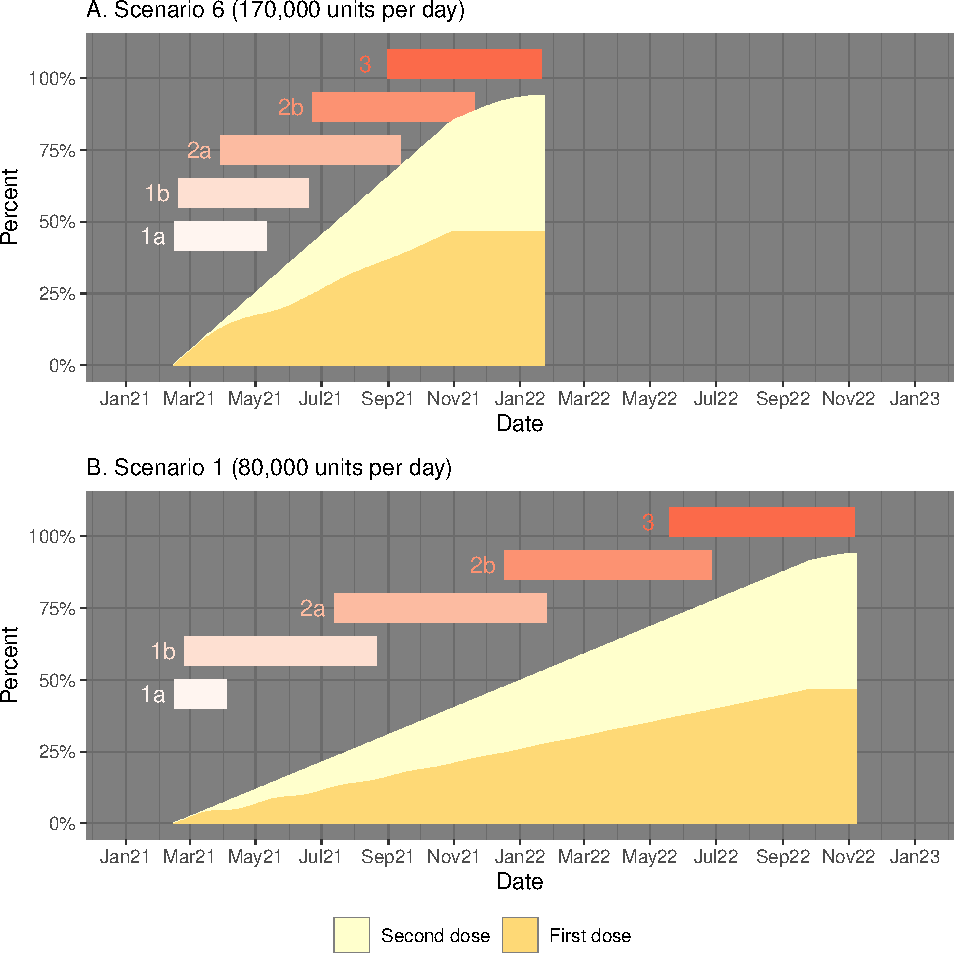
\includegraphics{researchNote_files/figure-latex/cumlResults-1} 

}

\caption{Cumulative vaccine doses over time}\label{fig:cumlResults}
\end{figure}

\hypertarget{discussion}{%
\section{Discussion}\label{discussion}}

To meet the target of vaccinating all adult Australians by the end of
October 2021 there will need to be, on average, in the order of 200,000
doses delivered daily (including weekends and holidays)--a truly furious
pace.

To test the feasibility of such a vaccination administration rate, it is
illuminating to consider the COVID-19 vaccination rates currently being
reported by other countries which have already begun to roll out their
vaccination programs (Figure \ref{fig:dailyVac}). The outlier is Israel,
where between 7,000 and 20,000 vaccinations per million population have
been delivered daily throughout January. Several factors may have
contributed to this success, including a young, largely urbanised
population and a strong public health infrastructure. Perhaps most
important has been strong logistical planning, including coordination of
delivery, ultra-cold-chain storage and staffing.\textsuperscript{9}
Other countries have been less successful in their roll-out to date,
including the United States (\textasciitilde4,000 per million pop max),
the United Kingdom (\textasciitilde5,000 per million pop max) and the
European Union (\textasciitilde1,100 per million pop max).

With a population of 25.7 million in Australia, the figure of 200,000
doses per day from our projections corresponds to approximately 7,800
daily doses per million population. Thus, it does seem possible to
vaccinate the Australian population in just eight months, but
administration rates considerably better than those currently being
achieved in most countries will be needed. Clearly Australia needs to
start as soon as possible, rapidly ramp-up to the required vaccination
velocity and then to maintain that relentless pace.

Apart from Phase 1a, currently announced delivery plans involve
recruiting, authorising and training 1,000 general practices and an
unknown number of pharmacies to administer vaccine doses, as well as
capture and record the required documentation for each
vaccinee.\textsuperscript{10} If authorised general practices alone are
relied upon to vaccinate the bulk of the population from Phase 1b
onwards, then on average each practice would need to administer 200
doses per day, seven days per week, for about six months. This seems
infeasible for all but the largest group practices. There are some 5,800
community pharmacies across Australia.\textsuperscript{11} If we assume
that half of these are willing and able to participate in the
vaccination programme, and each delivers an average of 35 doses per day
(including weekends and holidays), then this would represent half of the
daily administration capacity of 200,000 doses per day to meet the whole
of community vaccination target of the end of October 2021. However,
that still means that the 1,000 authorised general practices would need
to administer an average of 100 doses per day. This would still seem to
be a stretch, given that those practices would still have their normal
workloads to contend with. It seems clear that to deliver at the scale
needed will require dedicated large-scale vaccination sites that are
capable of delivering several thousands of doses a week, in addition to
the enthusiastic participation of GP practices and community pharmacies
around the country.

Of course, there are also major logistical challenges in ramping up such
a vaccination capacity. Adapting existing supply chain and vaccine
information systems to meet the demand is likely to take several weeks
at the most optimistic, and adequately training several clinical and
clerical staff from each of the authorised vaccination general practices
and pharmacies to safely screen patients, deliver the vaccines and
record the results is likely to take much longer than just one month.
Thus our assumption of commencement of vaccine roll-out at full
velocityby March 2021 seems particularly optimistic, and therefore the
estimates reported in the tables above are likely to be similarly
optimistic.

\begin{figure}

{\centering 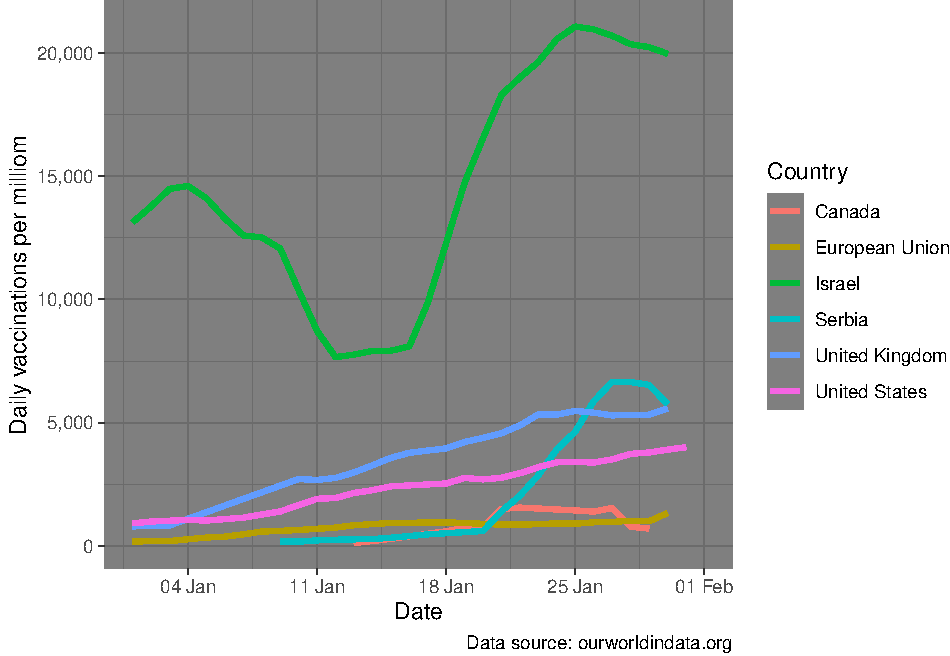
\includegraphics{researchNote_files/figure-latex/dailyVac-1} 

}

\caption{Daily COVID-19 vaccines administered per one million population}\label{fig:dailyVac}
\end{figure}

\hypertarget{acknowledgements}{%
\section{Acknowledgements}\label{acknowledgements}}

This research was supported by the generous assistance of Ian Sharp,
philanthropic supporter of UNSW research, and by a research seed grant
provided by the Sydney Partnership for Health, Education, Research and
Enterprise (SPHERE) Infectious diseases, Immunity and Inflammation
(Triple-I) Clinical Academic Group.

\newpage

\hypertarget{references}{%
\section*{References}\label{references}}
\addcontentsline{toc}{section}{References}

\hypertarget{refs}{}
\begin{cslreferences}
\leavevmode\hypertarget{ref-gh2021a}{}%
1. Health AGD of. Doorstop interview on 31 january 2021.
\emph{Australian Government Department of Health}. Published online
January 2021.
\url{https://www.health.gov.au/ministers/the-hon-greg-hunt-mp/media/doorstop-interview-on-31-january-2021}

\leavevmode\hypertarget{ref-rolloutStrategy}{}%
2. Australia's covid-19 vaccine national roll-out strategy. Published
online December 2020.
\url{https://www.health.gov.au/sites/default/files/documents/2021/01/australia-s-covid-19-vaccine-national-roll-out-strategy.pdf}

\leavevmode\hypertarget{ref-macdonald2015vaccine}{}%
3. MacDonald NE, others. Vaccine hesitancy: Definition, scope and
determinants. \emph{Vaccine}. 2015;33(34):4161-4164.

\leavevmode\hypertarget{ref-edwards2020covid}{}%
4. Edwards B, Biddle N, Gray M, Sollis K. COVID-19 vaccine hesitancy and
resistance: Correlates in a nationally representative longitudinal
survey of the australian population. \emph{medRxiv}. Published online
2020.

\leavevmode\hypertarget{ref-macintyre2020modelling}{}%
5. MacIntyre CR, Costantino V, Trent MJ. Modelling of covid-19
vaccination strategies and herd immunity, in scenarios of limited and
full vaccine supply in nsw, australia. \emph{medRxiv}. Published online
2020.

\leavevmode\hypertarget{ref-pm2021}{}%
6. Press conference - australian parliament house. Published online
January 2021.
\url{https://www.pm.gov.au/media/press-conference-australian-parliament-house-12}

\leavevmode\hypertarget{ref-R-base}{}%
7. R Core Team. \emph{R: A Language and Environment for Statistical
Computing}. R Foundation for Statistical Computing; 2019.
\url{https://www.R-project.org/}

\leavevmode\hypertarget{ref-tidyverse2019}{}%
8. Wickham H, Averick M, Bryan J, et al. Welcome to the tidyverse.
\emph{Journal of Open Source Software}. 2019;4(43):1686.
doi:\href{https://doi.org/10.21105/joss.01686}{10.21105/joss.01686}

\leavevmode\hypertarget{ref-mckee2021can}{}%
9. McKee M, Rajan S. What can we learn from israel's rapid roll out of
covid 19 vaccination? \emph{Israel Journal of Health Policy Research}.
2021;10(1):1-4.

\leavevmode\hypertarget{ref-gh2021b}{}%
10. Health AGD of. GPs' key role in covid-19 vaccination rollout.
\emph{Australian Government Department of Health}. Published online
January 2021.
\url{https://www.health.gov.au/ministers/the-hon-greg-hunt-mp/media/gps-key-role-in-covid-19-vaccination-rollout}

\leavevmode\hypertarget{ref-pga2020}{}%
11. Vital facts on community pharmacy. Published online December 2020.
\url{https://www.guild.org.au/__data/assets/pdf_file/0028/91909/PGA_December_2020_infographic.pdf}
\end{cslreferences}

\bibliographystyle{unsrt}
\bibliography{packages.bibreferences.bib}


\end{document}
